%*****************************************
\chapter{Introduction}\label{ch:introduction}
%*****************************************
    Neurons are capable of taking in, integrating, and outputting an enormous variety of information. Neurons can communicate information regarding everything ranging from motor behavior to complex sensory input, decision-making, and cognition. This requires neurons to be highly sensitive to internal cues such as intended modulation via biochemical and electrical pathways. On the other hand, neurons must maintain a consistent pattern of activity over a long timescale, despite high variability in intrinsic properties of neurons of the same type, and environmental perturbations such as ion channel turnover and activity perturbations. Neurons maintain this activity through homeostatic regulation, which is carried out through the use of neuromodulation and activity-dependent feedback\cite{liu_model_1998,lemasson_activity-dependent_1993,turrigiano_homeostatic_2004,cudmore_long-term_2004,desai_plasticity_1999,li_importance_2004,loebrich_function_2009,zhang_other_2003}.
    
    Previous work has described the existence of correlations between ion channel maximal conductances and channel mRNA concentrations in neurons\cite{schulz_variable_2006,schulz_quantitative_2007,golowasch_activity-dependent_1999}. Correlations are highly variable across neurons of the same cell type, but sets of correlations can be characterized to accurately predict the behavioral activity of a neuron. Correlations between ion channels have been shown to emerge from homeostatic tuning rules\cite{oleary_correlations_2013}, and may provide a mechanism by which homeostatic regulation can maintain consistent activity while neurons are undergoing ion channel turnover\cite{oleary_cell_2014}. However, it is currently unknown how homeostatic regulation can produce ion channel correlations. In this thesis, we will explore the possible mechanisms by which homeostatic tuning rules can produce ion channel correlations by modulating individual aspects of a model of homeostatic regulation.
    

%Biology
\section{Homeostasis} % need cute figures
Neurons maintain reliable patterns of activity despite high variability within neurons of the same type and a variety of external perturbations\cite{desai_plasticity_1999,golowasch_activity-dependent_1999,lemasson_activity-dependent_1993,turrigiano_activity-dependent_1994,turrigiano_selective_1995,turrigiano_homeostatic_1999,turrigiano_activity-dependent_1998}. For example, loss of neuromodulatory input is associated with changes in intrinsic membrane conductances which result in restoration of target firing rate activity\cite{turrigiano_activity-dependent_1994,turrigiano_selective_1995}.
Acting in synergy with their respective neuromodulatory environments, cells can stabilize activity over a long timescale\cite{franklin_long-term_1992,oleary_homeostasis_2010}.
The process of stabilizing electrical activity is undertaken by the use of compensatory mechanisms which make the neuron robust to perturbation. These mechanisms widen the range of characteristic sets of mRNA levels and conductance densities that produce desired activity\cite{rodgers_dopaminergic_2013,goldman_global_2001}.
Figure \ref{fig:golowasch1999} provides an example of this feature. For two different \ac{IC} neurons in the \acf{STG}, there exists significant variability between the two cells in their respective K\textsuperscript{+} currents and maximal conductance values. It can be seen here that individual channel maximal conductances vary several-fold in their respective densities. Despite this wide variation in ion channel maximal conductances, these neurons all produce the same patterns of activity.

\begin{figure}[h]
    \centering
    \includegraphics[width=\linewidth]{gfx/golowasch1999.png}
\caption[Variation in K\textsuperscript{+} currents and K\textsuperscript{+}-type maximal conductances in neurons in the \ac{STG}.]{\ac{IC} neurons in the \ac{STG} show significant variability in K\textsuperscript{+} currents and K\textsuperscript{+}-type channel maximal conductances\cite{golowasch_activity-dependent_1999}. (\textsc{A}) shows an example of three K\textsuperscript{+} currents in two different \ac{IC} neurons. (\texsc{B}) shows the mutual relationship between three different K\textsuperscript{+}-type channel maximal conductances. (\texsc{C}) Variation in conductance densities of K\textsuperscript{+}-type maximal conductances and the respective ratios between maximum and minimum conductance densities. (\textsc{D:}) Coefficient of variation (CoV) for the same K\textsuperscript{+}-type channel maximal conductances as in (\textsc{C:}). Figure reproduced from \cite{golowasch_activity-dependent_1999}.}
    \label{fig:golowasch1999}
\end{figure}

Previous work has shown that homeostasis in neurons can be regulated by a target level of excitability, which can be regulated by neuromodulation and activity-dependent feedback\cite{liu_model_1998,lemasson_activity-dependent_1993,turrigiano_homeostatic_2004, cudmore_long-term_2004, desai_plasticity_1999, li_importance_2004, loebrich_function_2009,, zhang_other_2003}.
Both mechanisms have been shown to be necessary for regulation of firing rate activity\cite{temporal_activity-dependent_2014}.
These mechanisms can change ion channel properties such as maximal conductance densities and mRNA transcript levels, in turn modulating firing rate activity\cite{zhang_other_2003,misonou_bidirectional_2006,daoudal_long-term_2003}.
Furthermore, the processes can modulate spatial distribution and localization of ion channels as well as associate channels with subunits that can further modify them\cite{shah_dendritic_2010,misonou_regulation_2004,marionneau_sodium_2012,kim_extended_2008}.

This thesis will utilize activity-dependent feedback as a homeostatic compensatory mechanism to explore the possible mechanisms which produce a wide variation in ion channel maximal conductances.
Activity-dependent feedback is premised on the idea that control of ion channel turnover must be regulated by a mechanism which is reliant on the firing properties of the neuron\cite{lemasson_activity-dependent_1993,liu_model_1998,stemmler_how_1999}. It has been shown to produce compensatory changes in ion channel maximal conductance densities and mRNA concentrations after prolonged changes in firing rate activity\cite{daoudal_long-term_2003,temporal_activity-dependent_2014,haedo_ionic_2006,turrigiano_activity-dependent_1994,turrigiano_selective_1995}.
This has been in observed in an experimental setting. For example, lobster \acs{STG} neurons which were chronically isolated from modulatory input recover endogenous bursting due to changes in intrinsic membrane conductances, indicating the presence of an activity-dependent mechanism\cite{turrigiano_activity-dependent_1994,turrigiano_selective_1995}.
Theoretical work has also shown that activity-dependent feedback can allow model neurons to produce complex patterns of activity starting from initial channel maximal conductances that produce quiescent behavior on their own\cite{oleary_correlations_2013,lemasson_activity-dependent_1993,liu_model_1998}.
These conductance-based models produce desired behavior via changes in conductance expression that are a result of activity-dependent cell-type specific channel expression rates.\cite{oleary_cell_2014}.

\section{Ion Channel Correlations}

Homeostatic regulation has been shown to produce diverse, highly variable correlations between ion channels\cite{schulz_variable_2006,schulz_quantitative_2007,golowasch_activity-dependent_1999}.
These correlations between ion channel maximal conductance densities and mRNA levels are found across phyla, and have shown to not be more similar within an animal than across a population, indicating genetic conservation of ion channel correlations\cite{tobin_correlations_2009,tran_ionic_2019}.

Examples of ion channel correlations are well documented within cell types and across species\cite{schulz_quantitative_2007,maclean_activity-independent_2003,santin_membrane_2019}. For example, correlations have been shown to exist in the \ac{CG}, as well as the \ac{STG} in crustaceans\cite{tobin_correlations_2009,baro_quantitative_1997,schulz_variable_2006,schulz_quantitative_2007}. 
Figure \ref{fig:santinschulz2019} shows a correlation network plot between thirteen different ion channel mRNAs in 11 \ac{PD} neurons in the \ac{STG}. Correlations are highly varied, exhibiting differences in connectivity and connection strengths between different mRNA levels.

\begin{figure}[h]
    \centering
    \includegraphics[width=\linewidth]{gfx/santinschulz2019.png}
    \caption[Correlations between 13 ion channel mRNAs in PD neurons.]{Correlation network plot of relationships between 13 ion channel mRNAs in eleven \ac{PD} neurons in the \ac{STG}. Correlations between ion channel mRNAs are shown to be vary significantly in connectivity and connection strength, indicated by the varying thickness of lines between ion channel mRNAs. (\textsc{C:}) Correlations between ion channel mRNAs in control. (\textsc{D:}) Correlations between ion channel mRNAs after 24 hours of tetrodotoxin (TTX) application. Correlations change significantly after application. Some relationships are totally lost (e.g. \textit{BKKCa} and \textit{Shaker}), while some are strengthened by application of TTX (e.g. \textit{CaV1} and \textit{Shab}). Figure reproduced from \cite{santin_membrane_2019}.}
    \label{fig:santinschulz2019}
\end{figure}

Along with that, changes in maximal conductances or mRNA levels of one ion channel can result in compensatory changes in others to preserve the activity of the neuron. For example, removal of \acs{ICa} causes compensatory decreases in \acs{IKCa} and \acs{IA} that are independent of kinetic channel properties\cite{peng_drosophila_2007}. 
Along with that, in the \ac{PD} neurons in the \ac{STG}, there exist strong correlations between channel conductance densities, as well as between mRNA levels, and the two have considerable overlap\cite{temporal_neuromodulation_2011}. %CITE TEMPORAL FIGURE
These findings exemplify that homeostatic regulation can produce ion channel correlations and that correlations can make the neuron robust to perturbation by providing a mechanism by which neurons can up- or down-regulate ion channels dependent on the activity of its correlated channels.

\subsection{Degeneracy}
%intro to degeneracy
%talk about schulz a lot
% figure from schulz
%back to ion channel correlations
Membrane channel mRNA levels and conductance density values can vary several-fold across cells of the same type\cite{schulz_variable_2006,liu_model_1998,golowasch_activity-dependent_1999,swensen_robustness_2005,prinz_similar_2004}.
It has been shown that this phenomenon occurs across species and types of neurons, ranging from neurons in the \ac{STG} to Purkinje cells in the cerebellum, and dopaminergic cells in the substantia nigra\cite{schulz_variable_2006,swensen_robustness_2005,liss_tuning_2001}.
For example, K\textsuperscript{+} currents in \ac{IC} neurons in \textit{Cancer borealis} display two- to five-fold variation in current densities\cite{golowasch_activity-dependent_1999}.
This indicates that neurons are degenerate with respect to patterns of activity -- behavioral patterns cannot be specified by a single set of maximal conductance densities or mRNA levels.
Rather, it has been shown that multiple sets of correlated ion channel mRNA levels and conductance densities can be characterized to identify neuronal cell types\cite{schulz_quantitative_2007,oleary_correlations_2013,oleary_cell_2014}.

From examination of these sets of parameters, it becomes clear that there are patterns of correlations between individual ion channels that are consistent across sets of ion channel maximal conductances and mRNA levels that produce the same patterns of activity. For example, \ac{gH} and \acf{gA} channel types consistently occur in a set ratio in their amplitudes\cite{maclean_activity-independent_2003,maclean_activity-independent_2005}. Along with that, \ac{PD} neurons and \ac{LP} neurons have been shown to possess correlated levels of \ac{gH}, \ac{gA}, and \ac{gKCa}, and are altered in a cell-specific manner by perturbation\cite{schulz_homeostatic_2017,temporal_neuromodulation_2011}.
Figure \ref{fig:goldman2005} shows the dependence of activity on both individual and subsets of ion channel maximal conductances. It can be seen that the same maximal conductance in one ion channel can result in different behavior depending on its relationship to maximal conductance densities of the other ion channels.

\begin{figure}[h]
    \centering
    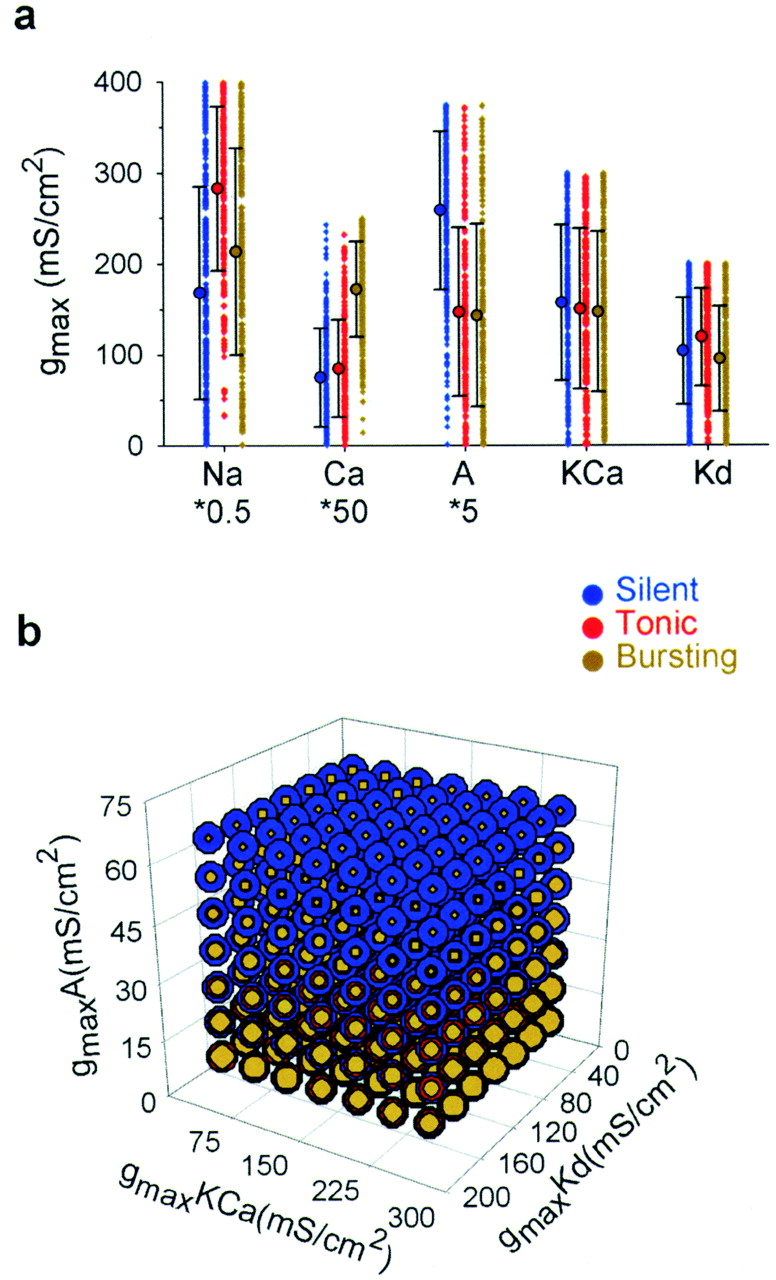
\includegraphics[scale=0.3]{gfx/goldman2001.jpg}
\caption[Dependence of different patterns of activity on ion channel relationships.]{Production of different patterns of activity in the neuron is dependent on the relationship between ion channel maximal conductances. The same maximal conductance density in one ion channel can produce unique patterns of activity dependent on its relationship to other channels. (\textsc{A:}) Different states of activity are observed when ion channel maximal conductances are varied over a wide range. (\textsc{B:}) Different patterns of activity emerge from characteristic sets of K\textsuperscript{+}-type ion channel maximal conductances in a probabilistic manner. The probability of seeing bursting activity, for example, increases as \ac{gA} and \ac{gKd} decrease toward zero\cite{goldman_global_2001}.}
    \label{fig:goldman2005}
\end{figure}

These patterns of correlations in channel expression and conductance density have been proposed reflect the tuning of conductances required to maintain target activity over a long period of time\cite{marder_variability_2006,schulz_variable_2006}.
This may arise during all periods of the life of a neuron, or it may be specific to initial development. In the \ac{STG}, it has been proposed that tuning rules governing development of neurons may result in networks that are highly variable across individuals by the time neural networks are fully developed\cite{marder_development_2005,rehm_spectral_2008,rehm_developmental_2008}.
Furthermore, variability in other systems may induce variability in ion channel expression and current densities -- the variability of transcriptional machinery and regulatory transcriptional sequences can lead to variability in gene transcription, and subsequently ion channel expression\cite{blake_noise_2003,volfson_origins_2006}.
It is currently unknown what biological mechanism, or mechanisms, produce variability across ion channel mRNAs and maximal conductance densities. Though neuroscience has come a long way in understanding how characteristic sets of ion channel mRNAs and maximal conductances can produce similar patterns of activity, we still do not know what drives the existence of these correlations\cite{prinz_similar_2004}.

\subsection{Homeostasis \& Ion Channel Correlations} \label{corr_homeostasis}
The existence of correlations between membrane ion channels may represent a mechanism by which homeostatic regulatory features may enforce and stabilize desired activity in specific neurons\cite{schulz_quantitative_2007}.
Co-regulation of ion channels can theoretically prevent loss of activity while the neuron is being affected by environmental perturbations such as ion channel turnover and activity perturbations\cite{oleary_correlations_2013,maclean_activity-independent_2003,bergquist_hierarchy_2010}.
Characteristic sets of ion channel correlations can consistently produce desired firing rate activity despite high variability in levels of channel conductance densities between individual neurons of the same cell type.
This has been proposed to occur through the enforcement of ion channel ratios, which are correlated to specific activity features. This can simplify homeostatic mechanisms and make the neuron robust to perturbations in any one ion channel\cite{schulz_quantitative_2007,maclean_activity-independent_2005,ball_coregulation_2010,burdakov_physiological_2005}.

Experimental work has shown ion channel correlations to be significantly affected by homeostatic activity\cite{taylor_axonal_2009,tran_ionic_2019,baumgardt_specification_2007,stein_modulation_2009,soofi_co-variation_2012,temporal_neuromodulation_2011}.
For example, MacLean \textit{et al.} showed that modulating \ac{gA} current densities or \ac{gH} current densities alone would change the functional output of the neuron, but that modulating both maintained desired functional output\cite{maclean_activity-independent_2005}.
Along with that, inhibition of \ac{gA} results in compensatory increase in \ac{gKCa} that is dependent on intracellular calcium concentration and calcineurin activity\cite{ransdell_rapid_2012}.
The dependence of this compensatory mechanism on calcium concentration provides evidence that activity-dependent feedback can influence ion channel correlations\cite{turrigiano_activity-dependent_1994,turrigiano_selective_1995}.

Though co-regulation of ion channels provides an avenue by which neurons may maintain desired activity, the mechanism which drives the existence of co-regulation remains a mystery.
Activity-dependent feedback represents but one proposed solution. The mechanism not only influences correlations, but is has been found necessary for the existence of correlated ion channels in the \ac{STG}.
Temporal \textit{et al.} performed experiments decoupling activity, synaptic connectivity, and neuromodulatory states of individual neurons from the \ac{STG}, and found that loss of neuromodulation was not sufficient to result in loss of correlations across channel mRNAs, but loss of activity resulted in loss of all correlations. Thus, it was shown that activity-dependent processes, but not neuromodulatory processes, can dynamically maintain distinct relationships across channel mRNAs in the \ac{STG}\cite{temporal_activity-dependent_2014}.
%TEMPORAL FIGURE
Activity-dependent feedback mechanisms can generate and regulate biophysically realistic dynamics of neurons in the \ac{STG}\cite{oleary_correlations_2013,oleary_cell_2014,liu_model_1998,lemasson_activity-dependent_1993}.
Figure \ref{fig:oleary2013} shows how a model of activity-dependent feedback (described in Section \ref{homeostaticrules}) can produce desired neuronal dynamics by varying channel conductances over time which are dependent on Ca\textsuperscript{2+} dynamics\cite{oleary_correlations_2013}.

\begin{figure}[H]
    \centering
    \includegraphics[width=1.0\linewidth]{gfx/oleary2013.png}
\caption[Model of activity-dependent feedback.]{Development of channel conductances and patterns of activity at different time-points. (\textsc{Left:}) A model of activity-dependent feedback varies channel conductances over time, resulting in desired functional output when channel conductances reach their respective steady-state values. (\textsc{Right:}) Patterns of activity (1-3) correspond to channel conductance values at three points in their evolution over time\cite{oleary_correlations_2013}.}
    \label{fig:oleary2013}
\end{figure}

These mechanisms are able to reliably influence co-regulation of ion channel pairs over different timescales by changing the properties of correlations, including slope, strength, and set-points within the parameter space\cite{stein_modulation_2009,soofi_co-variation_2012,temporal_neuromodulation_2011,tran_ionic_2019}.
%as you can see in this figure... from oleary et al 2013
The key feature of activity-dependent feedback is the dependence of functional output on firing rate activity. To sense changes in firing rate activity, models of activity-dependent feedback must have the capacity to sense these changes.
Calcium dynamics have been proposed as a way neurons can sense changes in activity. Calcium dynamics can indirectly express \ac{Vm} by simulating the interaction between changes in intracellular Ca\textsuperscript{2+} concentration and changes in \ac{Vm}.

Modern models of homeostasis typically use calcium dynamics as a sensor by which neurons can regulate activity\cite{turrigiano_activity-dependent_1994,turrigiano_selective_1995,oleary_correlations_2013,liu_model_1998}.
Changes in intracellular Ca\textsuperscript{2+} concentration can be averaged over different timescales in order to target different aspects of firing rate activity\cite{liu_model_1998}. In doing so, neurons can assure that functional output is properly maintained.
Liu \textit{et al.} described how different patterns of activity can have average Ca\textsuperscript{2+} concentration levels that may be difficult to differentiate between.

\begin{figure}[H]
    \centering
    \includegraphics[scale=0.7]{gfx/liu1998}
    \caption[Activity pattern differentiation in a single Ca\textsuperscript{2+} sensor setup.]{Three different patterns of activity have effectively equal average Ca\textsuperscript{2+}. (\textsc{A:}) \ac{Vm} of a neuron firing tonically. (\textsc{B:}) \ac{Vm} of a neuron firing with bursting behavior. (\textsc{C:}) \ac{Vm} of a neuron firing with a different bursting behavior. (\textsc{All, Right:}) Instantaneous Ca\textsuperscript{2+} concentration and respective time-averaged values\cite{liu_model_1998}.}
    \label{fig:liu1998}
\end{figure}

Figure \ref{fig:liu1998} shows that the Ca\textsuperscript{2+} average levels averaged over a single timescale across a tonic firing pattern and two separate bursting patterns are effectively equal. This shows that neurons which use a single Ca\textsuperscript{2+} sensor averaged over one unique timescale can, in theory and in some cases, not differentiate between different patterns of activity.
In contrast, Figure \ref{fig:liu1998_2} describes the use of three separate Ca\textsuperscript{2+} sensors which can distinguish between different activity patterns by averaging intracellular Ca\textsuperscript{2+} concentration over three distinct timescales.
The use of three sensors is not arbitrary in this case, but targets three key features of the neuron's electrophysiology. The fast Ca\textsuperscript{2+} sensor is able to detect tonic firing patterns, the slow Ca\textsuperscript{2+} sensor is able to detect bursting behavior, and the DC Ca\textsuperscript{2+} sensor can detect slow-wave activity.

\begin{figure}[H]
    \centering
    \includegraphics[scale=0.5]{gfx/liu1998_2.png}
    \caption[Activity pattern differentiation in a multiple Ca\textsuperscript{2+} sensor setup]{Three different Ca\textsuperscript{2+} sensors can differentiate between different patterns of activity. Rows \textsc{A-C} are the same activity patterns found in Figure \ref{fig:liu1998}. Second column shows Ca\textsuperscript{2+} current. Last three columns show transient and average values for three different Ca\textsuperscript{2+} sensors: Fast, Slow, and DC\cite{liu_model_1998}.}
    \label{fig:liu1998_2}
\end{figure}

Despite this, models of activity-dependent feedback have been produced which can differentiate between different patterns of activity, and reliably produce target behavior from initial conditions which produce quiescent behavior\cite{oleary_correlations_2013,oleary_cell_2014}. O'Leary \textit{et al.} has proposed a model which relies on a single Ca\textsuperscript{2+} sensor. At each discrete time-step, the difference, or "error," between the average Ca\textsuperscript{2+} concentration and the target Ca\textsuperscript{2+} concentration is computed, and integrated with past computations of error\cite{oleary_cell_2014}. This is then fed into two differential equations, one of which represents the synthesis of correlated ion channel mRNAs, and the other represents translation of ion channel proteins from the current channel mRNA concentration. This model scales the average Ca\textsuperscript{2+} concentration at the level of mRNA transcription, rather than at the level of the Ca\textsuperscript{2+} sensor. Ratios between ion channel maximal conductances can then specify correlations between conductances, and in turn specify the pattern of activity of the neuron. This model is shown to be a perfect candidate for exploring the effect of variability in other properties of the neuron on the variability of ion channel mRNA concentrations and maximal conductance densities.

Despite these significant achievements in producing biophysically realistic models of neuronal dynamics and homeostatic activity, ion channel correlations have nonetheless proven a significant challenge to models of neurons with homeostatic regulation. Sets of correlations are dissimilar across cell types and highly variable within cell types, making generalizability a challenge. Without an understanding of the functional mechanism driving their existence, or the biological mechanisms underlying activity-dependent feedback, creating biophysically realistic models is even more difficult\cite{schulz_quantitative_2007}.
The experimentally-derived correlations between ion channels have, as of now, not been successfully reproduced in models of homeostatic regulation\cite{schulz_variable_2006,schulz_quantitative_2007,oleary_correlations_2013,oleary_cell_2014,liu_model_1998}.
The model by O'Leary \textit{et al.} described above is capable of producing linear pairwise correlations between ion channel maximal conductances, but has not been able thus far to produce the non-binary patterns of correlations seen in Figure \ref{fig:santinschulz2019}\cite{oleary_cell_2014}.

In this thesis, variability in properties of model neurons including initial channel maximal conductances and mRNA levels, \acf{gleak}, \acf{taum}, \acf{taug}, and \acf{Ca_target} will be varied independently and systematically examined. The purpose in doing this is to understand the influence of intrinsic neural parameters and parameters of homeostatic regulation on emergence of ion channel correlations and the possible ways neurons can manifest ion channel correlations which are as diverse and robust as is seen in experimental observations.\cite{schulz_variable_2006,schulz_quantitative_2007}.

